\subsection{MB18 gas/spray penetration}
%%%%%%%%%%%%%%%%%%%%%%%%%%%%%%%%%%%%%%%
The primary concern of this project is fire modelling and suppression. In this \href{https://develop.openfoam.com/exafoam/wp2-validation/-/tree/master/lagrangian/sprayFoam/gasSprayPenetration?ref_type=heads}{MB18 gas/spray penetration testcase}, we deal with the main mechanism for fire suppression, namely via water spray, by which the liquid and evaporated species are mechanisms to reduce the enclosure temperature and/or directly to suppress the fire and source. This case uses the OpenFOAM Lagrangian solver to track the spray droplets trajectory through the mesh, coupled with the flow solver in exchange of mass (phase change), momentum (droplet and continuum fluid drag forces) and energy (needed to evaporate the liquid phase)

Validation of the following solvers within the Eulerian-Lagrangian framework
in terms of macroscopic and microscopic spray development and vaporisation:
\href{https://develop.openfoam.com/Development/openfoam/-/tree/master/applications/solvers/lagrangian/sprayFoam/sprayFoam.C}{sprayFoam}.

\subsubsection*{Methodology}
The test case is based on the Engine Combustion Network (ECN) workshop's \textit{Spray-A} experimental configuration \cite{ref1}. The \textit{Spray-A} case is a basic single-hole non-reacting spraying-into-a-closed-volume configuration; "well-characterized, but is likely non-cavitating (and thus, unrealistic)" \cite{ref2}.

\subsubsection*{Metrics}
The metrics to quantify the validations are \cite{ref3}:
\begin{itemize}
    \item Macroscopic spray development:
    \begin{itemize}
        \item Liquid penetration vs time (liquid-length)
        \item Vapor-phase penetration vs time
        \item Mixture fraction profiles (both axial and radial)
        \item Extinction profiles (both axial and radial)
    \end{itemize}
    \item Microscopic spray development:
    \begin{itemize}
        \item Spray penetration and velocity in the near-field
        \item Spreading angle
        \item Microscopic features (fuel ligaments, droplet formation etc.)
    \end{itemize}
\end{itemize}

\subsubsection*{Benchmarks}
The database of the experiments can be accessed through the \href{https://ecn.sandia.gov/ecn-data-search/}{ECN search engine}.

%The experimental configurations that were used in this study:
\begin{figure}[H]
    \centering
    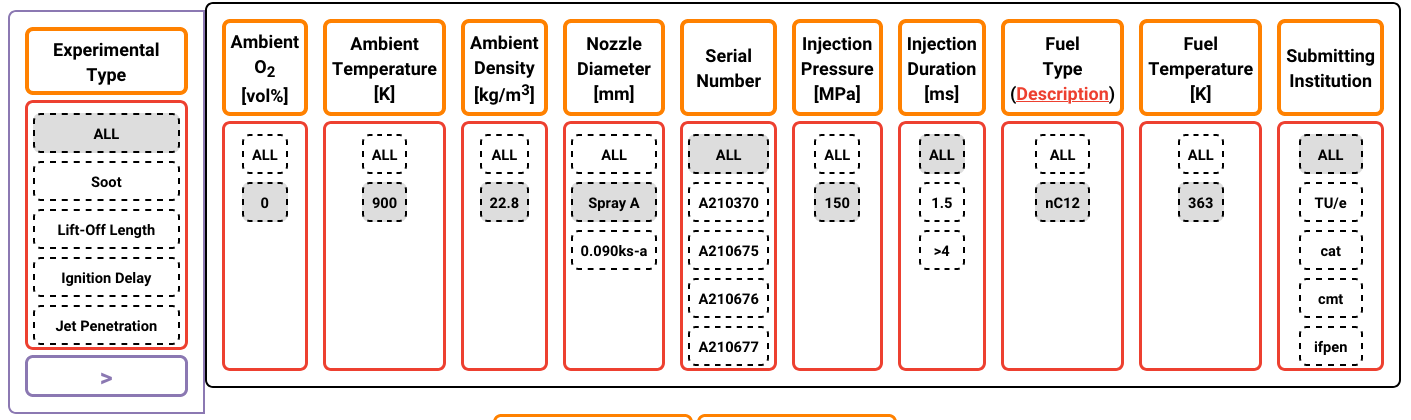
\includegraphics[width=0.9\linewidth]{figs/MB18/experiment-search-criteria.png}
    \caption{Experimental datasets used in this study.}
    \label{fig:enter-label}
\end{figure}

%The experimental datasets that were used in this study:
\begin{figure}[H]
    \centering
    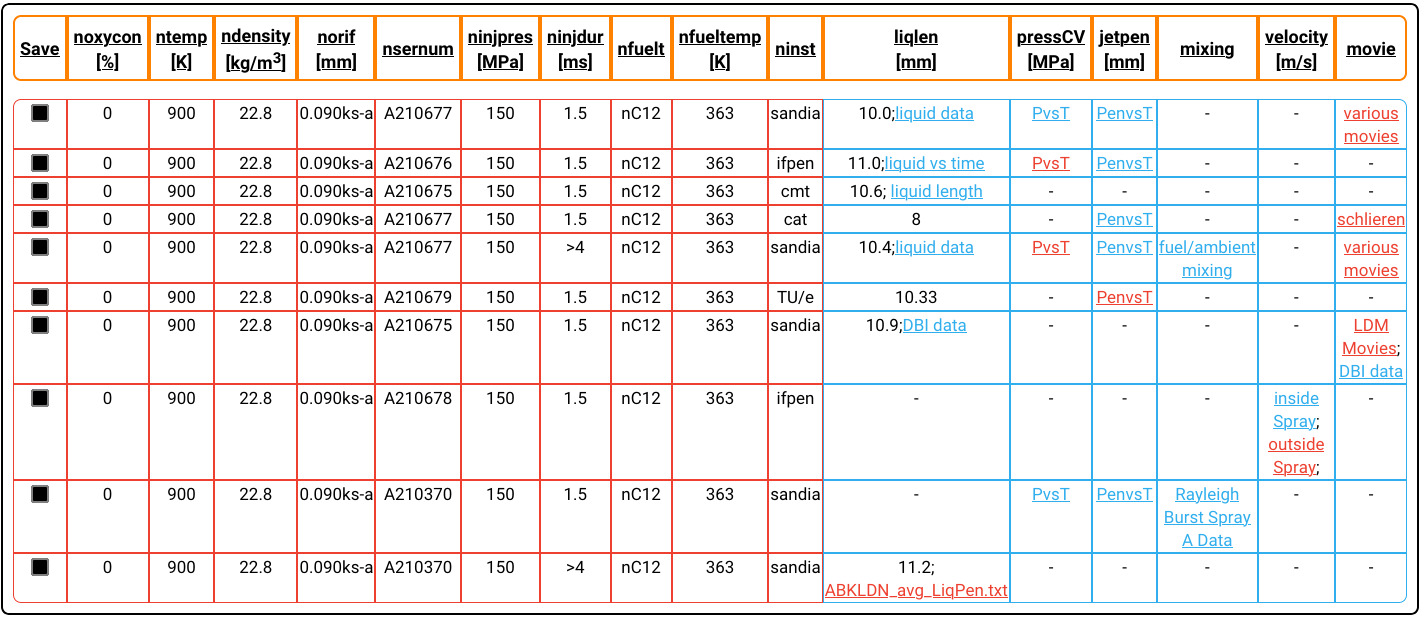
\includegraphics[width=0.9\linewidth]{figs/MB18/experiment-search-output.png}
    \caption{Experimental configurations used in this study.}
    \label{fig:enter-label}
\end{figure}

\subsubsection*{Definitions}
\paragraph{Liquid Penetration:} 
"Maximum distance from the nozzle outlet to the farthest axial position where projected liquid volume in the cross-stream direction decreases to a specific value. The projected liquid volume is defined as $\mathrm{PLV} = \int \mathrm{LVF} dy$, where $\mathrm{LVF}$ is liquid volume fraction and $\mathrm{PLV}$ is projected liquid volume. Two values for $\mathrm{PLV}$ are considered:" \cite{ref6}

\begin{equation}
    \int \mathrm{LVF} \, dy = 0.2\text{e-}3 \, [\mathrm{mm}^3 \, \text{liquid} / \mathrm{mm}^2]
\end{equation}

\begin{equation}
    \int \mathrm{LVF} \, dy = 2.0\text{e-}3 \, [\mathrm{mm}^3 \, \text{liquid} / \mathrm{mm}^2]
\end{equation}

In some studies, such as in \cite{ref7}, the liquid spray penetration "is defined as the maximum distance from the injector nozzle to the farthest axial position where 95\% of the liquid mass is found."

\paragraph{Vapor Penetration:} 
"Maximum distance from the nozzle outlet to where the fuel mass fraction (or mixture fraction (author's note: if the system is reacting)) is 0.1\%." \cite{ref6}

\subsubsection*{Physical Domain}
A constant volume vessel of cubic shape.

\subsubsection*{Physical Modelling}
Reference quantities \cite{ref1, ref7}:

\subsubsection*{Ambient Conditions (Gas)}
\begin{center}
\begin{tabular}{ll}
\hline
Metric & Value \\
\hline
Composition (by volume) & $0.00\%\,\mathrm{O}_2$, $6.52\%\,\mathrm{CO}_2$, $3.77\%\,\mathrm{H}_2\mathrm{O}$, $89.71\%\,\mathrm{N}_2$ \\
Temperature & $\mathrm{T}_{amb} = 900 \, [\mathrm{K}]$ \\
Pressure & $p_{amb} \approx 6.0 \, [\mathrm{MPa}]$ \\
Density & $\rho_{amb} = 22.8 \, [\mathrm{kg}/\mathrm{m}^3]$ \\
Velocity & Near-quiescent, less than $1 \, [\mathrm{m}/\mathrm{s}]$ \\
\hline
\end{tabular}
\end{center}

\subsubsection*{Injection Conditions (Liquid)}
\begin{center}
\begin{tabular}{ll}
\hline
Metric & Value \\
\hline
Fuel type & n-dodecane ($n\text{-}\mathrm{C}_{12}\mathrm{H}_{26}$) \\
Fuel temperature & $\mathrm{T}_{inj} = 363 \, [\mathrm{K}]$ \\
Density & $\rho = 713.13 \, [\mathrm{kg}/\mathrm{m}^3]$ \\
Injection duration(s) & $t_{inj} = 1.5 \, [\mathrm{ms}]$ and $t_{inj} = 6 \, [\mathrm{ms}]$ \\
Injection mass & $m_{inj} = 3.56 \, [\mathrm{mg}]$ \\
Injection pressure & $m_{inj} = 150 \, [\mathrm{MPa}]$ \\
Injection direction & Axial \\
Discharge coefficient & $c_{discharge} = 0.89 \, [-]$ \\
Mass flow rate of injection vs time & \href{resources/massFlowRateOfInjection_1.5}{1.5 ms} \\
\hline
\end{tabular}
\end{center}

Derived quantities \cite{ref7}:\\
\begin{center}
\begin{tabular}{ll}
\hline
Metric & Value \\
\hline
Turbulent kinetic energy & $k = 0.735 \, [\mathrm{m}^2/\mathrm{s}^2]$ \\
Turbulent kinetic energy dissipation rate & $\epsilon = 5.67 \, [\mathrm{m}^2/\mathrm{s}^3]$ \\
\hline
\end{tabular}
\end{center}

\subsubsection*{Spray Models}
The officially-recommended baseline spray models were reported in \cite{ref3, ref5}:

\begin{center}
\adjustbox{max width=\textwidth}{%
\begin{tabular}{ll}
\hline
Topic & Model \\
\hline
RANS closure model & RNG k-epsilon model \\
Injection & Blob injection \\
Atomisation and primary/secondary breakups & Kelvin-Helmholtz instability model and Rayleigh-Taylor accelerative instability mode (i.e., KHRT) \\
Collision & O'Rourke model \\
Drag & Dynamic model \\
Evaporation & Frossling model \\
Heat transfer & Ranz-Marshall model \\
Dispersion & Stochastic model \\
\hline
\end{tabular}}
\end{center}

The spray models being used in this study were listed as follows:

\begin{center}
\adjustbox{max width=\textwidth}{%
\begin{tabular}{ll}
\hline
Topic & Model \\
\hline
RANS closure model & RNG k-epsilon model \\
Injection & Injection: coneNozzleInjection Cone angle: $22^\circ$ \\
Atomisation and primary/secondary breakups & ReitzKHRT \\
Collision & None \\
Drag & sphereDrag \\
Evaporation & liquidEvaporationBoil \\
Heat transfer & RanzMarshall \\
Dispersion & stochasticDispersionRAS \\
Size distribution & Rosin Rammler \\
\hline
\end{tabular}}
\end{center}

\subsubsection*{Numerical Domain Modelling}
Dimensions: $(\mathrm{x}, \mathrm{y}, \mathrm{z}) = (180, 180, 180) \, [\mathrm{mm}]$

\begin{itemize}
    \item x: Longitudinal direction (mean spray direction)
    \item y: Spanwise direction
    \item z: Vertical direction
\end{itemize}

Injector characteristics:
\begin{itemize}
    \item Number of injector holes: 1 (axial)
    \item Nominal injector nozzle diameter: $D = 0.09 \, [\mathrm{mm}]$
\end{itemize}

\subsubsection*{Numerical Domain Discretisation}
Spatial domain discretisation: See \texttt{system/blockMeshDict}. (nref=1)

\begin{itemize}
    \item $\Delta x_{min} = 0.25 \, [\mathrm{mm}]$ (in spray liquid core region)
    \item $\Delta x_{max} = 4.0 \, [\mathrm{mm}]$
\end{itemize}

\begin{figure}[H]
    \centering
    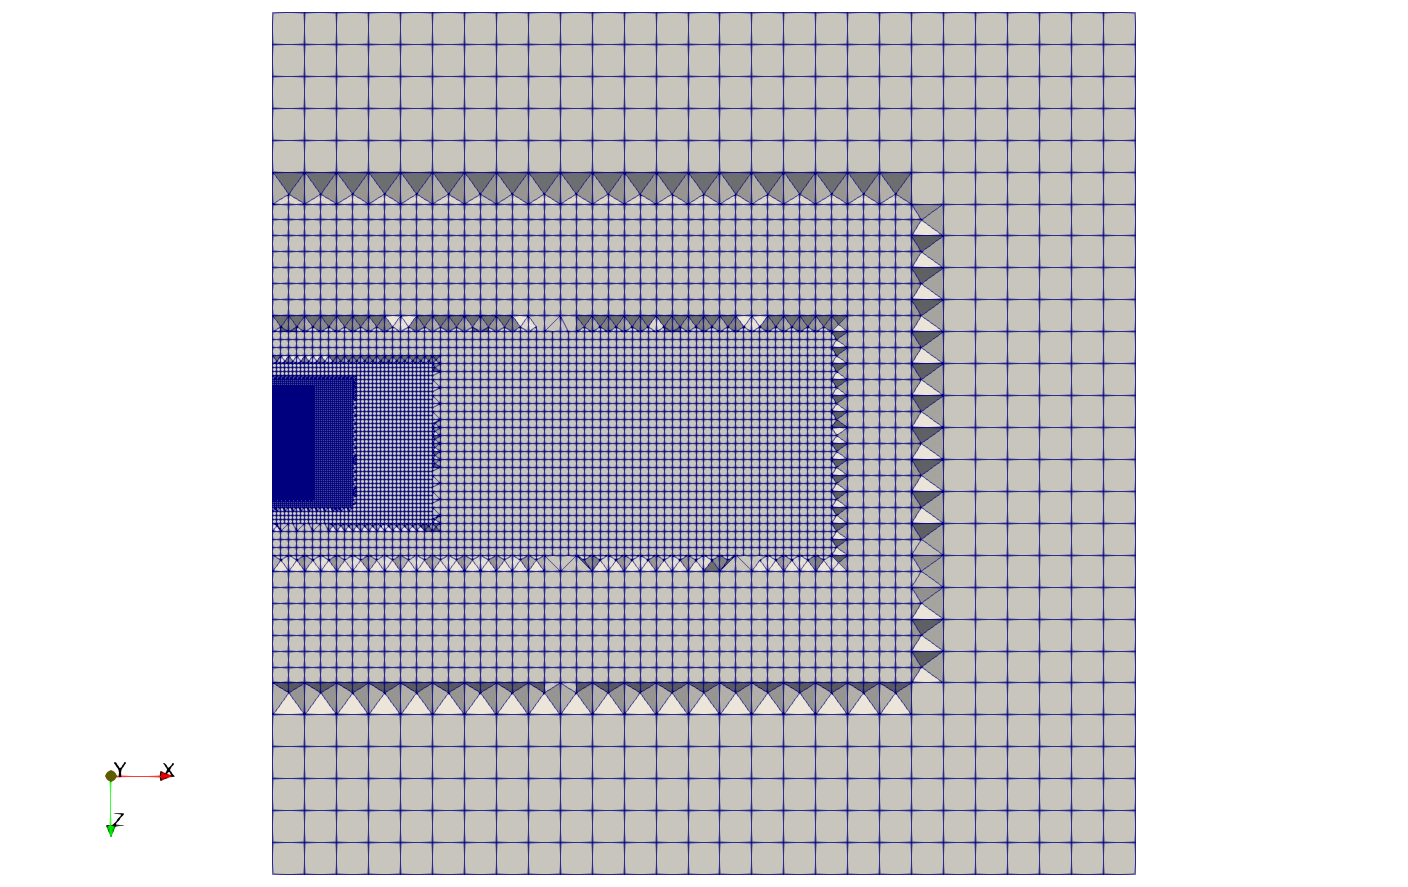
\includegraphics[width=\linewidth]{figs/MB18/side-view-mesh.png}
    \caption{Spatial domain discretisation.}
    \label{fig:enter-label}
\end{figure}

Coaxial-cylindrical refinement regions with respect to the injector nozzle centre (i.e., $(0 0 0)$), progressively finer towards the injection hole (nref=1):

\begin{center}
\begin{tabular}{llll}
\hline
Refinement level & Size [mm] & Radius [mm] & Height [mm] \\
\hline
0 & 4.0 & - & - \\
1 & 2.0 & 30 & 80 \\
2 & 1.0 & 15 & 70 \\
3 & 0.5 & 10 & 20 \\
4 & 0.25 & 8 & 10 \\
5 & 0.125 & 7 & 5 \\
\hline
\end{tabular}
\end{center}

Temporal resolution:
\begin{itemize}
    \item $\Delta t_{min} = 5\text{e-}7 \, [\mathrm{s}]$
    \item $\Delta t_{min} = 2\text{e-}7 \, [\mathrm{s}]$
\end{itemize}

\subsubsection*{Equation Discretisation}
\begin{itemize}
    \item Spatial derivatives and variables: See \texttt{system/fvSchemes}.
    \item Temporal derivatives and variables: See \texttt{system/fvSchemes}.
\end{itemize}

\subsubsection*{Numerical Boundary/Initial Conditions}
Refer to \texttt{0.orig}.

\subsubsection*{Pressure-Velocity Coupling Algorithm}
PISO.

\subsubsection*{Linear Solvers}
Refer to \texttt{system/fvSolution}.

\subsubsection*{Initialisation and Sampling}
No initialisation/averaging. Refer to \texttt{system/controlDict} for function objects being used.

\subsubsection*{Instructions to Run the Case}
The setup for nref=1 (baseline) is tested in OpenFOAM v2206. Execution is typically a call to Allrun script with required number of processors as argument. e.g., \texttt{./Allrun 16}.

\subsubsection*{Results}
%\paragraph{Liquid Penetration vs Time}
\begin{figure}[H]
    \centering
    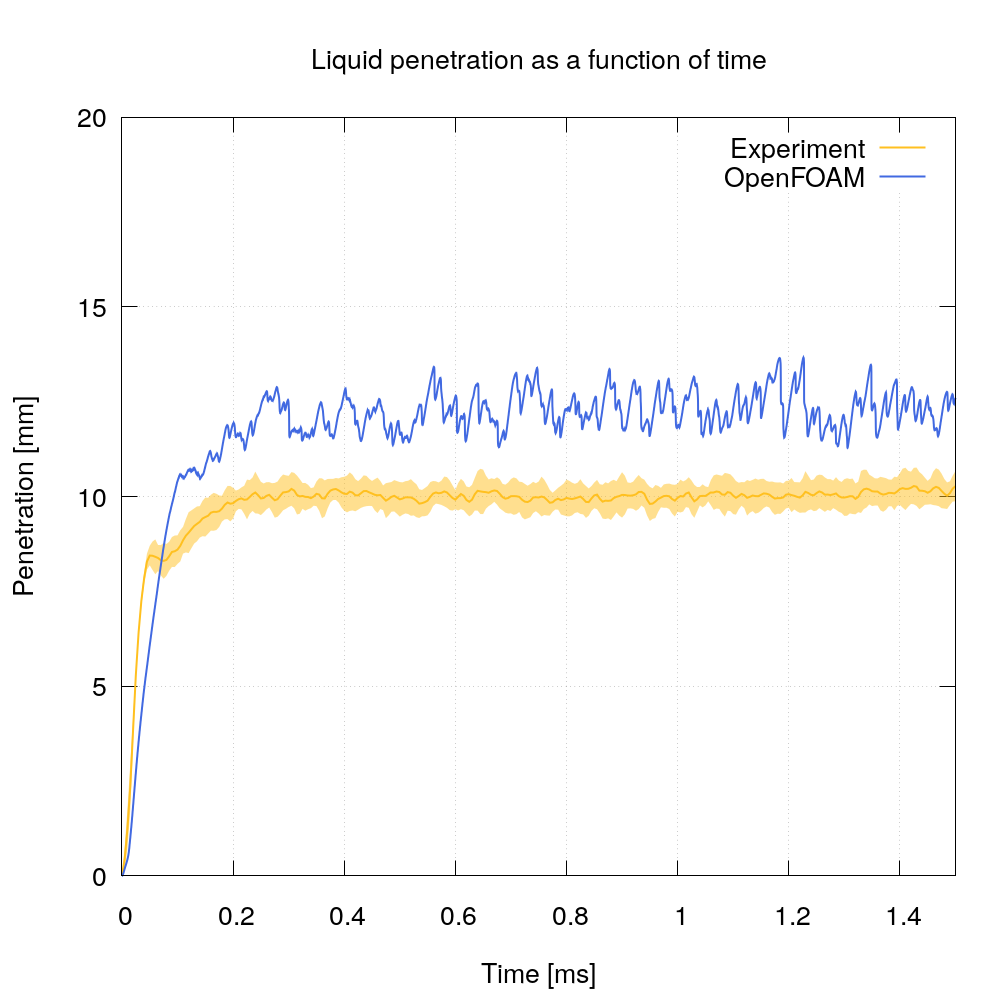
\includegraphics[width=0.9\linewidth]{figs/MB18/liquid_penetration.png}
    \caption{Liquid Penetration vs Time.}
    \label{fig:enter-label}
\end{figure}

%\paragraph{Vapor-phase Penetration vs Time}
\begin{figure}[H]
    \centering
    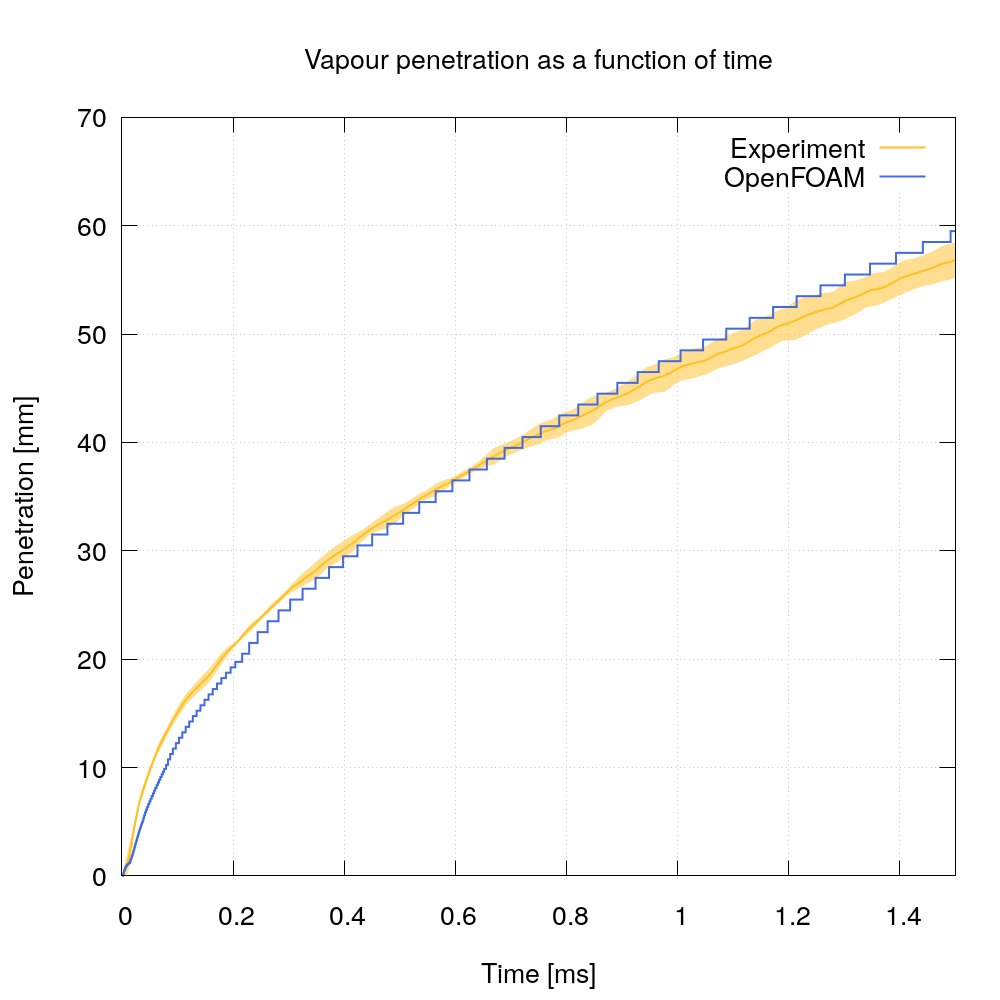
\includegraphics[width=0.9\linewidth]{figs/MB18/vapour_penetration.png}
    \caption{Vapor-phase Penetration vs Time.}
    \label{fig:enter-label}
\end{figure}

\subsubsection*{Bottlenecks}
The bottlenecks to be addressed in exaFOAM using the release code series OpenFOAM-vYYMM are:
\begin{itemize}
    \item Scalability of combined flow and Lagrangian OpenFOAM solvers
    \item Computational load between the continuum and discrete particle solvers (number of particles versus mesh count).
    \item Load-balancing and performance benchmarking as the Lagrangian particles transport in space.
\end{itemize}

\subsubsection*{Discussion}
\begin{itemize}
    \item The breakup model constant $B_1$ has a significant impact on the spray modeling, since it controls the diameter reduction of secondary droplets.
    \item In general, given a set of spray model parameters, the simulation results are not grid independent.
    \item Note that these gas velocities are small when compared to liquid (high-momentum) spray velocities (400 to 600 m/s) and therefore, have little effect on the sprays.
    \item The effect of URANS turbulence models on liquid penetration is not pronounced.
    \item Conversely, there is a significant discrepancy among the vapor penetration predictions over time.
\end{itemize}
